\documentclass[tikz,border=5pt]{standalone}
% Shared pastel academic grammar for final-size technical-paper diagrams.
\usepackage[T1]{fontenc}
\usepackage{lmodern}
\usepackage{amsmath,amssymb}
\usepackage{xcolor}
\usepackage{tikz}
\usetikzlibrary{
  arrows.meta,
  backgrounds,
  calc,
  circuits.logic.US,
  decorations.pathreplacing,
  fit,
  matrix,
  patterns,
  positioning,
  shapes.geometric,
  shapes.symbols
}

\definecolor{ink}{RGB}{24,24,28}
\definecolor{midink}{RGB}{96,96,104}
\definecolor{paleink}{RGB}{184,184,190}
\definecolor{wash}{RGB}{241,240,237}
\definecolor{paper}{RGB}{255,255,253}
\definecolor{cyan}{RGB}{126,203,218}
\definecolor{cyanwash}{RGB}{211,238,242}
\definecolor{pink}{RGB}{235,139,158}
\definecolor{pinkwash}{RGB}{250,211,217}
\definecolor{purple}{RGB}{166,50,150}
\definecolor{purplewash}{RGB}{232,196,227}
\definecolor{gold}{RGB}{177,139,45}
\definecolor{goldwash}{RGB}{239,226,183}
\definecolor{slate}{RGB}{116,133,145}
\definecolor{slatewash}{RGB}{221,226,229}
\colorlet{muted}{midink}
\colorlet{rule}{paleink}
\colorlet{accent}{purple}
\colorlet{accentwash}{purplewash}
\colorlet{second}{cyan}
\colorlet{secondwash}{cyanwash}

\tikzset{
  every picture/.style={
    font=\rmfamily\footnotesize,
    text=ink,
    line cap=round,
    line join=round,
    >=Stealth
  },
  every node/.style={outer sep=0pt},
  panel mark/.style={font=\rmfamily\bfseries\footnotesize},
  primary/.style={font=\rmfamily\footnotesize},
  secondary/.style={font=\rmfamily\scriptsize,text=midink},
  signal name/.style={font=\ttfamily\footnotesize,anchor=east},
  scope trace/.style={draw=ink,line width=.62pt,line cap=butt,line join=miter},
  hairline/.style={draw=paleink,line width=.28pt,line cap=butt},
  dotted guide/.style={draw=midink,line width=.32pt,densely dotted},
  dashed scope/.style={draw=ink,line width=.45pt,dashed},
  transition/.style={-{Stealth[length=1.8mm,width=1.25mm]},draw=ink,line width=.58pt},
  transition label/.style={font=\rmfamily\scriptsize,fill=paper,inner sep=1.2pt},
  preedge/.style={circle,draw=ink,fill=paper,line width=.58pt,minimum size=8.2mm,inner sep=1pt},
  observed preedge/.style={preedge,fill=purplewash,double,double distance=1.15pt,line width=.62pt,minimum size=9.8mm},
  brace/.style={decorate,decoration={brace,mirror,amplitude=3pt},draw=ink,line width=.45pt},
  grid rule/.style={draw=slate,line width=.32pt,line cap=butt},
  outer rule/.style={draw=ink,line width=.82pt,line cap=butt,line join=miter},
  star mark/.style={star,star points=5,star point ratio=2.2,draw=ink,fill=purple,minimum size=5.1mm,inner sep=0pt},
  % Compatibility vocabulary used by the repository's other figures.
  flow/.style={-{Latex[length=4.5pt,width=3.2pt]},draw=ink,line width=.55pt},
  heavy flow/.style={-{Latex[length=5pt,width=3.6pt]},draw=ink,line width=.8pt},
  wire/.style={draw=ink,line width=.5pt},
  bus/.style={draw=ink,line width=1.05pt},
  guide/.style={draw=midink,line width=.4pt,dotted},
  alternate/.style={draw=ink,line width=.5pt,dashed},
  scope/.style={draw=ink,line width=.5pt,dashed,inner sep=6pt},
  block/.style={draw=ink,line width=.55pt,fill=paper,minimum height=8mm,inner xsep=5pt,inner ysep=4pt,align=center},
  operation/.style={block,fill=cyanwash,minimum width=17mm},
  register/.style={block,fill=paper,minimum width=16mm,minimum height=10mm},
  state/.style={circle,draw=ink,line width=.55pt,fill=cyanwash,minimum size=8mm,inner sep=1pt,align=center},
  terminal/.style={state,fill=purplewash,double,double distance=1.2pt,line width=.6pt},
  predicate/.style={diamond,aspect=1.8,draw=ink,line width=.55pt,fill=pinkwash,inner xsep=3pt,inner ysep=2pt,align=center},
  datum/.style={rectangle,draw=ink,line width=.5pt,fill=goldwash,minimum width=8mm,minimum height=6mm,inner sep=2pt,align=center},
  panel label/.style={font=\rmfamily\bfseries\footnotesize},
  local heading/.style={font=\rmfamily\bfseries\footnotesize},
  annotation/.style={font=\rmfamily\scriptsize,text=midink,align=center},
  heading/.style={font=\rmfamily\bfseries\small},
  subheading/.style={font=\rmfamily\bfseries\footnotesize},
  note/.style={font=\rmfamily\scriptsize,text=midink},
  label/.style={font=\rmfamily\bfseries\scriptsize},
  mono/.style={font=\ttfamily\footnotesize},
  tiny mono/.style={font=\ttfamily\scriptsize},
  count/.style={font=\rmfamily\bfseries\small},
  selected/.style={draw=ink,fill=purplewash,line width=.8pt},
  cell on/.style={fill=purple,draw=ink,line width=.3pt},
  cell off/.style={fill=paper,draw=paleink,line width=.3pt}
}

% Flat pastel facets and depth edges for restrained axonometric constructions.
\tikzset{
  cyan facet/.style={draw=ink,fill=cyanwash,line width=.5pt,line join=round},
  cyan side/.style={draw=ink,fill=cyan,line width=.5pt,line join=round},
  pink facet/.style={draw=ink,fill=pinkwash,line width=.5pt,line join=round},
  pink side/.style={draw=ink,fill=pink,line width=.5pt,line join=round},
  purple facet/.style={draw=ink,fill=purplewash,line width=.55pt,line join=round},
  purple side/.style={draw=ink,fill=purple,line width=.55pt,line join=round},
  gold facet/.style={draw=ink,fill=goldwash,line width=.5pt,line join=round},
  gold side/.style={draw=ink,fill=gold,line width=.5pt,line join=round},
  context facet/.style={draw=ink,fill=slatewash,line width=.45pt,line join=round},
  depth edge/.style={draw=midink,line width=.38pt},
  surface grid/.style={draw=slate,line width=.32pt},
  projection/.style={draw=midink,line width=.38pt,densely dashed},
  accent curve/.style={draw=purple,line width=1.05pt},
  cyan curve/.style={draw=cyan!70!ink,line width=.9pt},
  pink curve/.style={draw=pink!70!ink,line width=.9pt},
  gold curve/.style={draw=gold!80!ink,line width=.9pt}
}


\tikzset{
  coordinate index/.style={font=\rmfamily\scriptsize,text=ink},
  tally cell/.style={
    font=\rmfamily\bfseries\scriptsize,
    text=ink,
    minimum width=5.3mm,
    minimum height=5.3mm,
    inner sep=0pt
  },
  figure note/.style={font=\rmfamily\scriptsize,text=ink,align=center},
  small heading/.style={font=\rmfamily\bfseries\footnotesize,text=ink,align=center}
}

\begin{document}
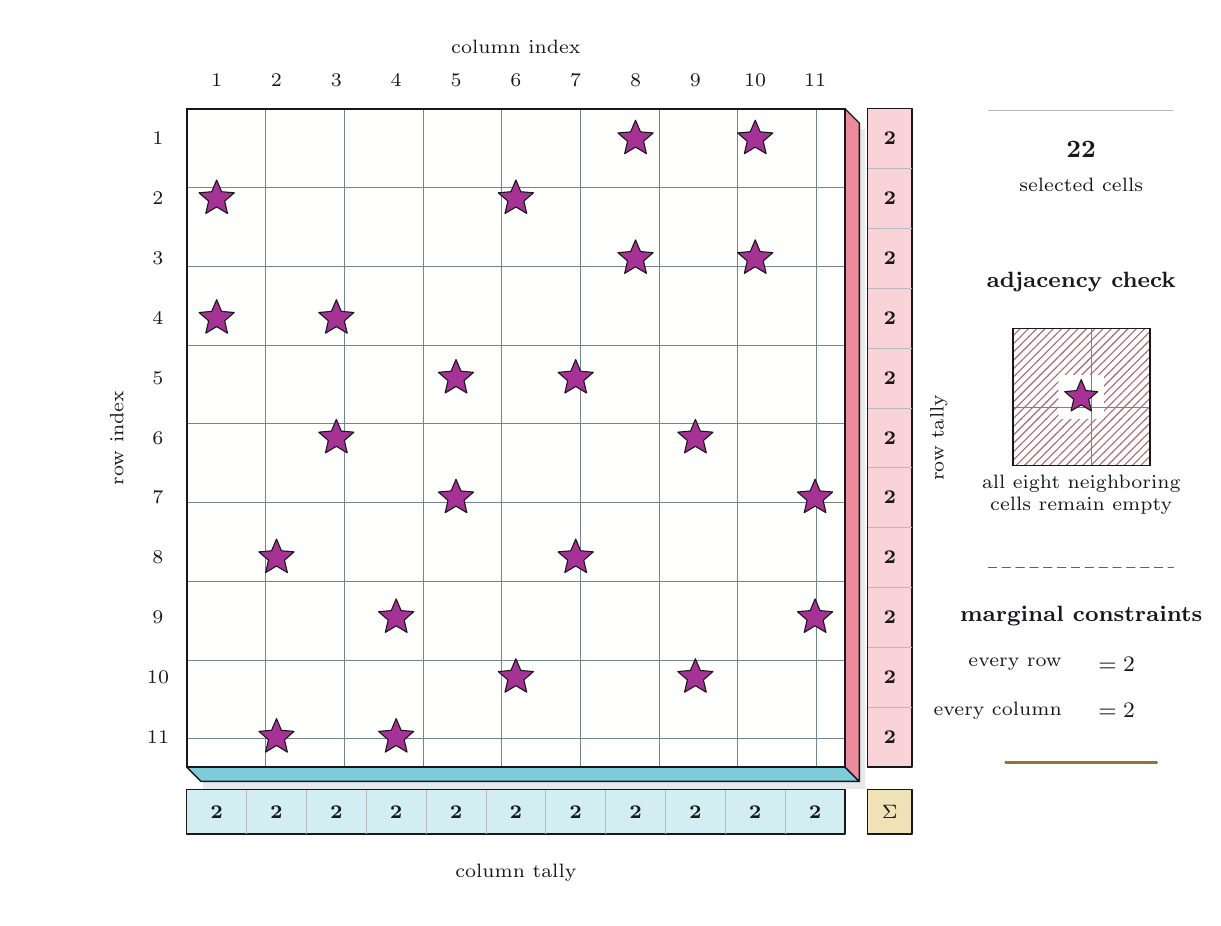
\begin{tikzpicture}[x=1cm,y=1cm]
  \path[use as bounding box] (0,0) rectangle (14.8,11.05);

  % The face remains orthographic; only its lower and right edges carry depth.
  \begin{scope}[shift={(2.02,10.02)},x=.76cm,y=-.76cm]
    \path[fill=slate!18,draw=none]
      (.28,.34) rectangle (11.34,11.37);
    \path[cyan side]
      (0,11) -- (11,11) -- (11.24,11.24) -- (.24,11.24) -- cycle;
    \path[pink side]
      (11,0) -- (11.24,.24) -- (11.24,11.24) -- (11,11) -- cycle;
    \path[fill=paper,draw=ink,line width=.68pt] (0,0) rectangle (11,11);

    % Marginal projections distinguish counts from coordinate indices.
    \path[cyan facet,fill=cyanwash]
      (0,11.38) rectangle (11,12.12);
    \path[pink facet,fill=pinkwash]
      (11.38,0) rectangle (12.12,11);
    \path[gold facet,fill=goldwash]
      (11.38,11.38) rectangle (12.12,12.12);
    \foreach \k in {1,...,10}{
      \draw[hairline] (\k,11.38) -- (\k,12.12);
      \draw[hairline] (11.38,\k) -- (12.12,\k);
    }

    \foreach \c in {1,...,11}{
      \node[coordinate index] at ({\c-.5},-.48) {\c};
      \node[tally cell] at ({\c-.5},11.75) {2};
    }
    \foreach \r in {1,...,11}{
      \node[coordinate index] at (-.48,{\r-.5}) {\r};
      \node[tally cell] at (11.75,{\r-.5}) {2};
    }
    \node[font=\rmfamily\bfseries\scriptsize] at (11.75,11.75) {$\Sigma$};

    \draw[grid rule] (0,0) grid (11,11);
    \draw[outer rule] (0,0) rectangle (11,11);

    % Exact row-major placement from solution_bits.txt: 22 stars total.
    \foreach \c/\r in {
      8/1,10/1,
      1/2,6/2,
      8/3,10/3,
      1/4,3/4,
      5/5,7/5,
      3/6,9/6,
      5/7,11/7,
      2/8,7/8,
      4/9,11/9,
      6/10,9/10,
      2/11,4/11
    }{
      \node[star mark,minimum size=4.7mm] at ({\c-.5},{\r-.5}) {};
    }
  \end{scope}

  \node[figure note,anchor=south] at (6.20,10.60) {column index};
  \node[figure note,rotate=90] at (1.13,5.84) {row index};
  \node[figure note,anchor=north] at (6.20,.55) {column tally};
  \node[figure note,rotate=90] at (11.57,5.84) {row tally};

  % A compact structural certificate: hatch, not hue, marks forbidden neighbors.
  \draw[hairline,line width=.4pt] (12.20,10.00) -- (14.55,10.00);
  \node[count] at (13.38,9.50) {22};
  \node[figure note] at (13.38,9.05) {selected cells};

  \node[small heading] at (13.38,7.82) {adjacency check};
  \begin{scope}[shift={(12.51,7.23)},x=.58cm,y=-.58cm]
    \path[fill=paper] (0,0) rectangle (3,3);
    \foreach \x/\y in {0/0,1/0,2/0,0/1,2/1,0/2,1/2,2/2}{
      \path[fill=pinkwash,pattern=north east lines,pattern color=pink!70!ink]
        (\x,\y) rectangle ++(1,1);
    }
    \draw[grid rule,line width=.35pt] (0,0) grid (3,3);
    \draw[outer rule,line width=.62pt] (0,0) rectangle (3,3);
    \node[star mark,minimum size=4.4mm] at (1.5,1.5) {};
  \end{scope}
  \node[figure note] at (13.38,5.12)
    {all eight neighboring\\cells remain empty};

  \draw[projection] (12.20,4.20) -- (14.55,4.20);
  \node[small heading] at (13.38,3.58) {marginal constraints};
  \node[figure note,anchor=east] at (13.25,2.96) {every row};
  \node[font=\rmfamily\bfseries\footnotesize,anchor=west] at (13.48,2.96) {$=2$};
  \node[figure note,anchor=east] at (13.25,2.38) {every column};
  \node[font=\rmfamily\bfseries\footnotesize,anchor=west] at (13.48,2.38) {$=2$};
  \draw[gold curve] (12.42,1.72) -- (14.34,1.72);
\end{tikzpicture}
\end{document}
